\section{Fast Detector Simulation}\label{sec:ml4sim}

\subsection{Background}\label{subsec:simbkg}

Full detector simulation using \GEANTfour~\cite{Agostinelli:2002hh} is highly accurate, but computationally costly:
it consumed 40\% of grid CPU usage by the major LHC experiments during Run 2~\cite{Apostolakis:2018ieg}.
This limits the number of simulated events that can be produced, directly increasing uncertainties and reducing sensitivity.
In particular, SVJ searches (Section~\ref{sec:darkqcd}) require large background samples to design optimal strategies
and large signal samples for thorough scans of all of the signal model parameters.
However, \textbf{statistical uncertainty in simulation impacts the entire collider physics program}, including measurements of the Higgs boson.

\begin{figure}[htb!]
\centering
\twofigeqh{figures/cpu_cms2022.pdf}{figures/cpu_pie_cms2022.pdf}
\caption{Left: projected CPU needs will exceed available resources for CMS in Run 3 (LHC) and Runs 4--5 (HL-LHC) without substantial R\&D.
Right: proportions of CPU usage by activity during Run 4, showing reconstruction (RECO and RECOSIM) as the largest, while simulation (SIM) remains the second-largest.
Reproduced from Ref.~\cite{CMS-NOTE-2022-008}.
}
\label{fig:cmsoffcomp}
\end{figure}

The severity of this problem will increase dramatically for the HL-LHC, which will provide an order of magnitude more data,
along with growth in per-event complexity from the associated detector upgrades.
Figure~\ref{fig:cmsoffcomp} illustrates the extreme computing challenges in the HL-LHC era.
The proportion of computing used for reconstruction increases because of superlinear scaling of key algorithms with the number of collisions per event.
Reconstruction has received substantial attention and effort to pursue algorithmic and technical improvements,
such as GPU implementations of tracking and pulse shape fitting already deployed by CMS in Run 3~\cite{Bocci:2020pmi}.
However, the challenges facing simulation have been relatively underserved;
it remains the second-largest contributor after reconstruction, so dedicated, coordinated effort is needed.
The CPU time used by the full detector simulation is expected to increase by a factor of 3 or more~\cite{Pedro:2020kbk},
because the detector upgrades introduce more complex geometries and higher precision requiring more detailed physics models.

The CMS detector simulation already benefits from numerous technical optimizations and physics-preserving approximations,
which improve its CPU efficiency by a factor of 4--6 compared to baseline \GEANTfour, as demonstrated by the PI~\cite{Pedro:2019mkq}.
The PI also led the effort to integrate a modernized CPU-based simulation engine in the CMS software (CMSSW)~\cite{Pedro:2020kbk},
which achieved a factor of 2 speedup~\cite{Amadio:2020ink}.
He now consults on the implementation of the GPU-based simulation engine Celeritas~\cite{Tognini:2022nmd} in CMS;
this project offers promising gains in simplified examples, but its performance with the full CMS geometry and physics interactions has yet to be established.
\textbf{Generative AI offers an alternative and complementary approach to achieve substantial speedups using GPUs, highlighted in the recent DOE report}~\cite{AI4SES}.

\subsection{Objectives}\label{subsec:simobj}

In order for a generative AI algorithm to become a broadly useful replacement for full detector simulation,
it must provide a similar level of quality while substantially increasing computational efficiency.
The PI formed and leads the CMS Machine Learning for Simulation (ML4Sim) group, and previously convened the HEP Software Foundation Detector Simulation Working Group
and the Theoretical Calculations and Simulation topical group for the Snowmass Computational Frontier~\cite{Boyle:2022cvo,Elvira:2022wyn}.
Through these roles, he is directing the field toward an emphasis on practical usability of generative AI:
the desired level of quality must be reached in order for any increase in computational speed to be meaningful.
Recently, diffusion models have come to dominate generative tasks in industry, such as the popular text-to-image generators Stable Diffusion, DALL${\cdot}$E, and Midjourney.
The PI has demonstrated that diffusion models can produce simulations of the necessary quality in public datasets~\cite{Amram:2023onf},
exceeding the performance of other approaches~\cite{Adelmann:2022ozp,Hashemi:2023rgo}.

We will now apply diffusion models to simulate particle showers in the CMS calorimeters, which are the major contributor to increasing per-event simulation time at the HL-LHC~\cite{Pedro:2020kbk}.
We pursue two complementary paths for the AI algorithms (1, 2), both deployed in the same way (3):
\begin{enumerate}
\item the ``fully generative'' approach, producing showers from completely random input (Section~\ref{subsec:diffu});
\item the ``hybrid'' approach, producing showers from approximately correct input (Section~\ref{subsec:refine});
\item integrate in the experiment software using the ``inference as a service'' approach (Section~\ref{subsec:iaas}).
\end{enumerate}
We target percent-level agreement with \GEANTfour and at least a factor of 100 improvement in throughput by using GPU coprocessors.
Both are achievable given existing results, with further increases to the speed of diffusion expected as part of the project.
Any remaining discrepancies between the full and AI-based simulations will be handled by an existing, simpler form of the hybrid approach~\cite{Bein:2023ylt}.
\textbf{The readiness of the entire AI-based CMS simulation chain before the HL-LHC startup will facilitate the Run 3 capstone dark QCD scan, as well as all future Run 4 activities.}

The impact of AI-based simulation will be felt even at colliders beyond the HL-LHC.
P5 has recommended~\cite{P5:2023} an increase in R\&D toward future higher-energy colliders
to further our exploration of the universe, including the nature of dark matter.
In particular, the report highlights a muon collider as a path to 10\TeV parton center-of-mass energy, potentially at Fermilab.
\textbf{Simulation studies are one of the first critical items to understand the feasibility and design of the muon collider and its detectors.}
These simulations face an even greater challenge: the beam-induced background (BIB), from muon decays in flight, produces unprecedented particle multiplicity
such that a single event currently takes 24 hours to simulate in \GEANTfour.
A combination of the Celeritas GPU-based classical simulation engine and AI-based simulation using diffusion models will be necessary to handle the BIB at scale.
Delivering this application by the end of the grant will help ensure the success of the next generation of collider experiments.

\subsection{Step 1: Fully Generative AI-based Simulation}\label{subsec:diffu}

Diffusion models are a type of generative AI, inspired by the physical process of diffusion.
Starting from some input data, such as images or calorimeter showers,
a training dataset is built by deterministically adding different amounts of randomness to each image.
Because the amount of randomness in each training image is known, the diffusion model can learn how to perform the addition of randomness to any data.
The objective of the model is simply a regression task, and therefore the training converges reliably.
Figure~\ref{fig:illus} shows how adding randomness repeatedly, over many iterations, produces an image that is purely random.
To generate new images, this process is reversed, starting from pure randomness to produce realistic data (``denoising'').

\begin{figure}[htb!]
\centering
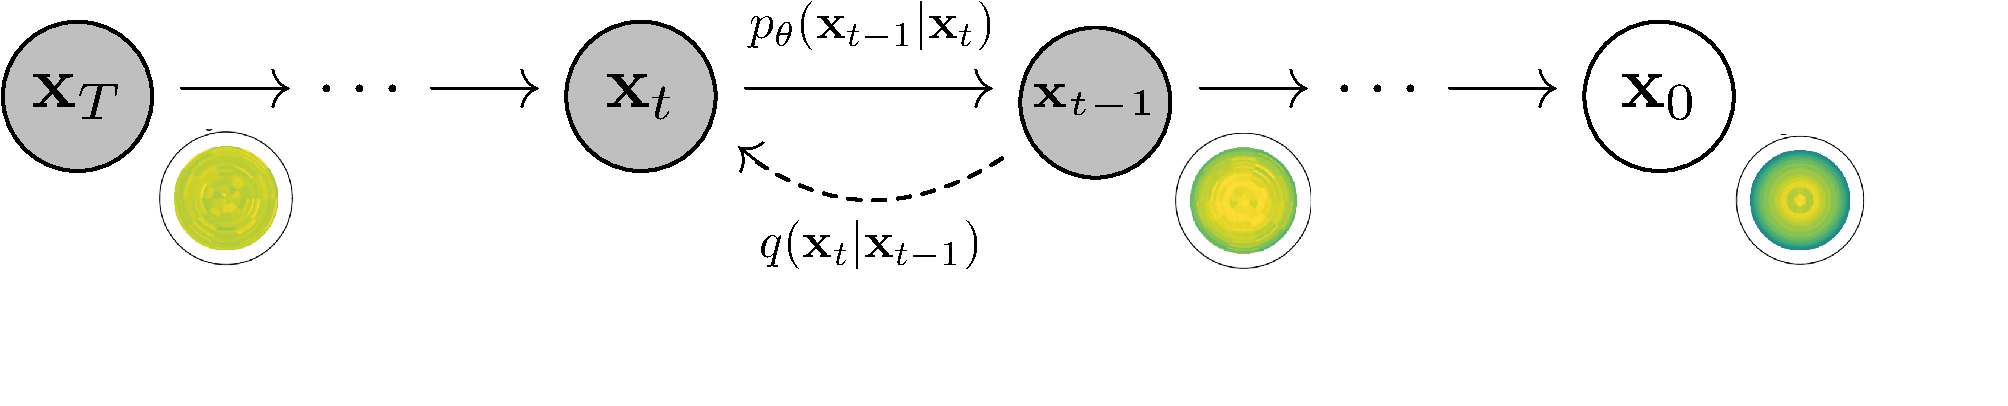
\includegraphics[width=0.95\myfigurewidth]{figures/pgm_diagram_xarrow_showers.pdf}
\caption{An illustration of the diffusion process, going from pure randomness (left) to a realistic particle shower (right) in a transverse slice of a calorimeter. Adapted from Ref.~\cite{Ho:2020}.}
\label{fig:illus}
\end{figure}

The PI and his team developed the \diffu algorithm for the \challenge,
a recent community effort to compare different AI approaches to the simulation of particle showers in calorimeters, using common datasets and metrics~\cite{CaloChallenge}.
The datasets include sampling calorimeters with varying materials and granularities and different particles including photons, pions, and electrons.
\diffu uses convolutional operations, which are computationally efficient because they share parameters and act on local data.
Several novel geometric adaptations were developed to help the convolutions handle non-rectangular and irregular calorimeter geometries.
Figure~\ref{fig:calodiffu} (left) shows results from the \challenge on the pion dataset, \textbf{clearly demonstrating the superiority of \diffu,
which is found to produce the highest quality showers for all datasets}~\cite{Krause:2023mlj}.
The algorithms are compared based on metrics including classifier scores and the Fr\'echet particle distance~\cite{Kansal:2022spb}.
This version of the algorithm is published in Ref.~\cite{Amram:2023onf};
subsequently, the quality has been improved even further, as shown in Fig.~\ref{fig:calodiffu} (right), by adding a separate module that learns the per-layer deposited energy.

\begin{figure}[htb!]
\centering
\twofigeqh{figures/ds1-pions_CE_1.pdf}{figures/FCC_ERatio_dataset2_oct11_layer_norm_Diffu.pdf}
\caption{Left: example comparison of the separation power (a $\chi^2$-like measure of the similarity between distributions~\cite{Diefenbacher:2020rna})
from the shower center of energy between AI algorithms and \GEANTfour in the community \challenge, adapted from Ref.~\cite{Krause:2023mlj}.
\diffu has the lowest values, showing that it is almost identical to \GEANTfour.
Right: The total deposited energy for the improved version of \diffu compared to \GEANTfour.}
\label{fig:calodiffu}
\end{figure}

\textbf{Here, we propose to adapt \diffu to the more complex and variable CMS geometry.}
First, we will adapt the model to the existing, simpler CMS calorimeters,
in order to deliver the necessary simulation for the dark QCD scan (Section~\ref{subsec:darkscan}).
This also serves as a useful intermediate step toward the most involved case,
the High Granularity Calorimeter (HGCal), a part of the HL-LHC detector upgrades
that will increase the number of channels by almost two orders of magnitude.
The HGCal will have both hexagonal and rectangular cells in different regions, with different material types and thicknesses.
It is also the major driver of the predicted increase in \GEANTfour simulation time~\cite{Pedro:2020kbk}.
Further optimizations of the \diffu model will be needed to handle the high dimensionality and precision requirements of this new detector.

\diffu runs 10-100 times faster than \GEANTfour by processing particles in large batches on GPUs.
While the initial version required 400 denoising iterations or ``steps'' to produce high-quality output,
the improved version requires a factor of 4--8 fewer steps, depending on the dataset, because of its intrinsically higher quality.
More recently, some of the PI's colleagues have used \diffu as a platform to test further improvements to both the training and inference~\cite{Jiang:2024ohg},
and the most promising of these have been integrated into the model~\cite{Amram:GitHub}.
Numerous other avenues to make the algorithm faster while preserving quality are under investigation~\cite{Rombach:2022,Song:2023,Mei:2023}.
These illustrate a critical advantage of diffusion models:
\textbf{because of the massive interest in these models in the broader ML community and in industry,
new methods are constantly being developed that can be easily imported for HEP use cases,}
relying on the collaborative nature of open-source software.

\textit{Risk mitigation}: if the various approaches to speed up the fully generative diffusion model do not succeed,
this will reduce the amount of simulation that can be produced,
though we still expect to exceed \GEANTfour when running in batches on GPU.
Based on existing results, the fully generative diffusion model will almost certainly produce higher quality output than existing fast simulation (FastSim) approaches in CMS~\cite{Sekmen:2016iql}.
However, if it does not, Section~\ref{subsec:refine} includes alternative approaches to improve the existing FastSim.

\subsection{Step 2: Hybrid Simulation}\label{subsec:refine}

\begin{wrapfigure}[21]{L}{0.5\textwidth}
\centering
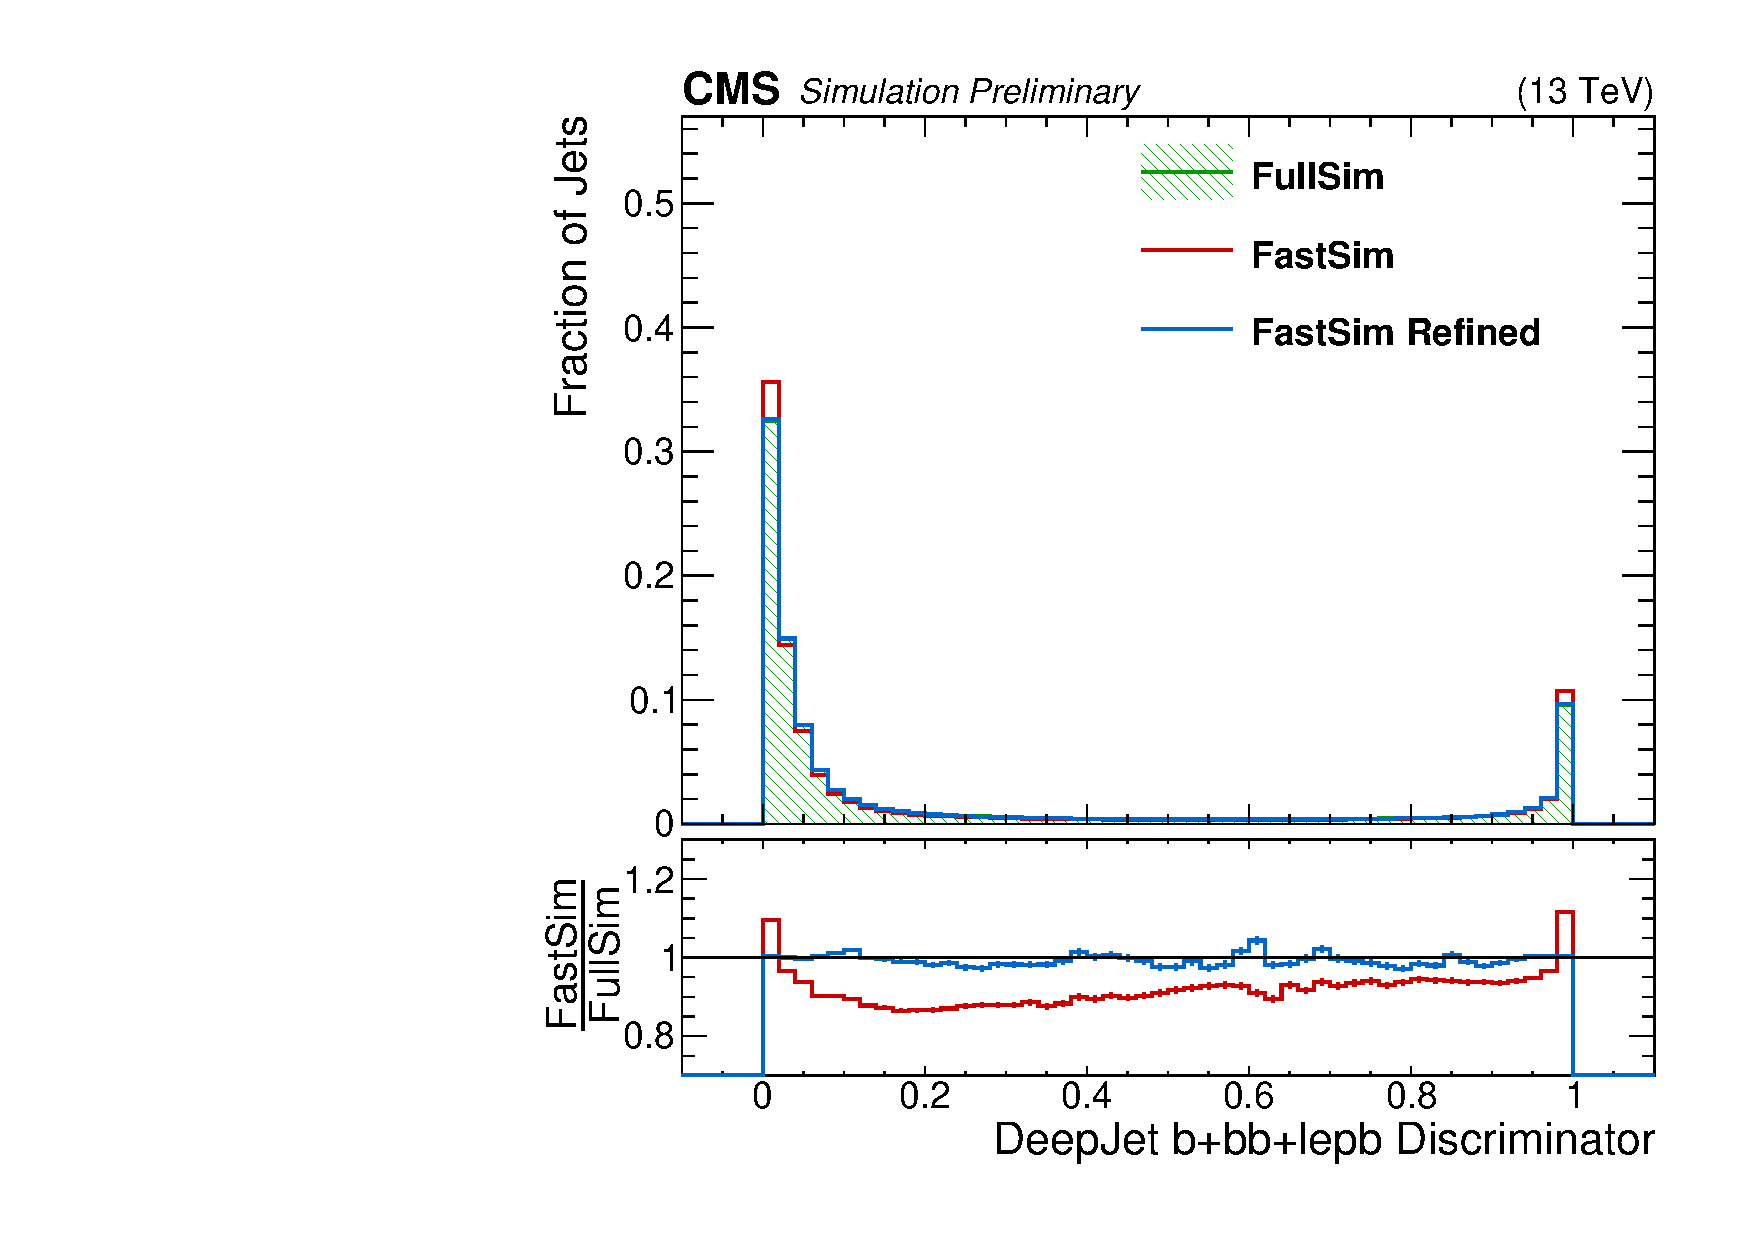
\includegraphics[width=0.49\myfigurewidth]{figures/Regression_20221127_DeepFlavB_preliminary.pdf}
\caption{The distribution of the \DEEPJET \cPqb-jet tagging discriminator: FastSim deviates from \GEANTfour by ${\sim}10\%$, while refined FastSim has percent-level agreement with \GEANTfour.}
\label{fig:refine}
\end{wrapfigure}

Refining a low-quality simulation to obtain high-quality output was the objective of the PI's previous denoising project, which used a less sophisticated AI architecture~\cite{Banerjee:2022gkg}.
Diffusion models are much more capable, but so far the ``fully generative'' approach (producing a shower from pure randomness) has been pursued;
this is because the sampling algorithms applied during the inference steps rely on the Gaussian nature of the randomness.
The differences between FastSim and \GEANTfour will not be Gaussian, so while it is easier in principle to learn the difference between two similar distributions,
additional mathematical formalism must be derived in order to reuse the existing diffusion approach.
Ref.~\cite{Mei:2023} provides an alternative approach to achieve the same goal:
\textbf{feeding information from FastSim into the fully generative model in order to guide the diffusion to generate high-quality output in just one inference step}.

The PI and his team have also developed a complementary high-level refinement, directly targeting analysis-level variables~\cite{Bein:2023ylt}.
With promising results on \cPqb-jet tagging variables, shown in Fig.~\ref{fig:refine},
the algorithm is now being expanded to other jet-related variables and validated for use in Run 3.
The approach can be understood as a significantly more precise, correlation-preserving alternative to traditional, manually-calculated correction factors.
Given that the CMS FastSim currently only agrees with \GEANTfour to within ${\sim}10\%$,
\textbf{high-level refinement alone can substantially reduce the quality deficits in FastSim samples and the resulting uncertainties.}

The combination of diffusion and refinement will be even more powerful.
In the chain FastSim~$\to$~diffusion~$\to$~refinement, each ML algorithm solves a progressively easier problem,
because the difference with respect to the previous step is smaller.
Therefore, it can learn the solution more precisely from a given dataset size,
as well as incorporating physics at different levels: individual detector hits and reconstructed kinematic variables.
\textbf{Refinement will address any residual disagreements between FastSim-based \diffu and \GEANTfour,
resulting in a more accurate final product}, much like next-to-leading order matrix element calculations increase in accuracy by incorporating higher-order effects.

\textit{Risk mitigation}: if methods to combine the diffusion model with the existing FastSim do not succeed,
we can use the fully generative diffusion model or high-level refinement alone, at the cost of reduced computing speed or increased uncertainty, respectively.

\subsection{Step 3: Inference as a Service}\label{subsec:iaas}

AI algorithm inference uses a restricted set of operations, such as matrix multiplications, which can naturally be accelerated on coprocessors.
The PI is the lead developer for the Services for Optimized Network Inference on Coprocessors (SONIC) approach, which implements inference as a service.
SONIC allows seamless utilization of coprocessors in experiment software, with demonstrated inference speedups of multiple orders of magnitude,
for CMS, ATLAS, the Deep Underground Neutrino Experiment (DUNE), the Laser Interferometer Gravitational-Wave Observatory (LIGO), and analysis facilities~\cite{Duarte:2019fta,Krupa:2020bwg,Wang:2020fjr,Rankin:2020usv,Gunny:2021gne,Cai:2023ldc,CMS:2024twn,Savard:2023wwi}.
The underlying framework takes advantage of open-source tools, including the Nvidia Triton inference server~\cite{nvidia} and advances in machine learning packages.

The latest results for SONIC in CMS are shown in Fig.~\ref{fig:sonic}:
ParticleNet inference throughput can be increased up to a factor of 100 by using GPUs with the optimal backend software configuration~\cite{CMS:2024twn}.
This approach essentially eliminates the impact of AI algorithm inference on event throughput,
and the use of asynchronous, non-blocking requests~\cite{Bocci:2020olh} further eliminates the impact of latency when connecting to remote coprocessors,
at least up to a distance of hundreds of kilometers.
A single coprocessor, located anywhere, can serve tens or even hundreds of CPU processes.
SONIC has already been shown to work with GPUs, FPGAs, TPUs (tensor processing units), and IPUs (intelligence processing units).

\begin{wrapfigure}[19]{r}{0.5\textwidth}
\centering
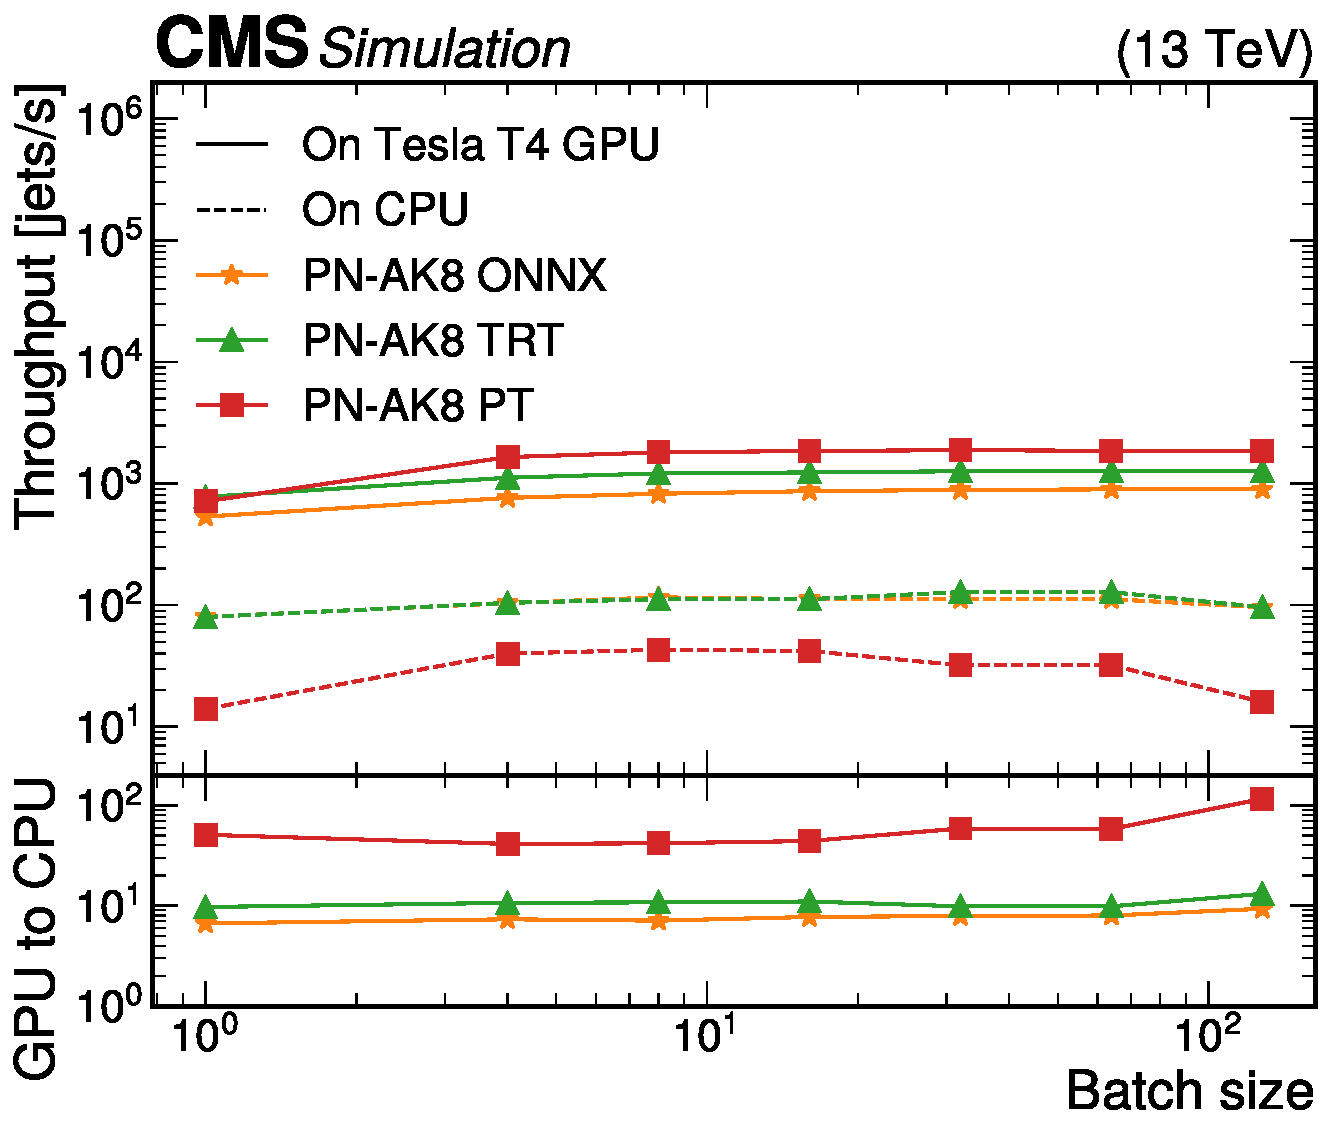
\includegraphics[width=0.49\myfigurewidth]{figures/CMS-MLG-23-001_Figure_005-b.pdf}
\caption{The inference throughput for ParticleNet on CPU and GPU, using ONNX, TensorRT, and PyTorch backends. PyTorch on GPU provides the largest throughput increase.}
\label{fig:sonic}
\end{wrapfigure}

As noted in Section~\ref{subsec:diffu}, the maximum speedup for AI-based simulation is achieved by performing inference on GPU
and generating showers for at least 100 particles simultaneously.
In order to reliably fill the GPU register memory, particles from multiple events must be processed together.
In addition, most CPUs in the Worldwide LHC Computing Grid currently are not directly connected to GPUs.
These considerations point to SONIC as the right approach to integrate AI-based simulation into experiment software frameworks.
\textbf{The PI has nearly unparalleled expertise in implementing simulation engines and inference as a service in experiment software},
through his previous roles in CMS software management and current role as lead developer of SONIC.
Deploying AI-based simulation via SONIC provides a path for efficient utilization of HPC resources and even new, unforeseen coprocessors.

\textit{Risk mitigation}: if unforeseen complications are encountered in the use of inference as a service,
directly-connected GPUs can be employed, at the cost of limiting the computing sites where simulation can be run effectively.

\textbf{The final product of this work is an AI-augmented simulation engine
that carries out rule-based algorithms on local CPUs and AI inference on remote GPUs via SONIC.}
A common implementation for diffusion model inference will be shared between the \GEANTfour and CMS FastSim interfaces to ensure consistency and minimize the maintenance burden.
Implementation in the experiment software is critical to validate the performance of either the fully generative or hybrid approach.
This requires comparisons of reconstruction-level quantities that can only be computed using the entire CMSSW processing chain.
The technologies and innovations in this part of the proposal have mostly been proven to work in other contexts, as shown above.
Viable alternatives exist to mitigate the risks from the new elements.

\subsection{Future Colliders}\label{subsec:mucoll}

If a hidden valley exists but only couples to the SM via mediators at the 10\TeV scale, collider DM production will require a future, higher energy accelerator.
The new P5 report~\cite{P5:2023} specifically highlights a muon collider as an attractive option to reach parton center-of-mass energies of 10\TeV,
both because of its compact footprint and because of the numerous technological innovations and synergies that would be achieved in the course of constructing and operating this machine.
\textbf{While the collider itself is several decades away, the report highlights that research into its feasibility must start now.}
Simulation is a crucial component of the design process for both the detectors and the collider,
and the machine-detector interface (MDI) is particularly important for the muon collider.
The MDI must incorporate mitigations for the beam-induced background (BIB) caused by muon decays in flight as the beam circulates.
At $\sqrt{\smash[b]{s_{\Pgm\Pgm}}} = 10\TeV$, there are ${\sim}10^5$ muon decays per meter, leading to ${\sim}10^8$ photons and neutrons per bunch crossing~\cite{Black:2022cth}.

Currently, it takes 24 hours to simulate just one BIB event with \GEANTfour.
AI-based BIB simulation, therefore, would be highly impactful for muon collider, detector, and MDI design.
While \diffu is trained on single-particle events, because material interactions in \GEANTfour are modeled independently for every particle,
it may not be feasible to continue such an approach for events with $10^8$ particles.
If so, we will implement a ``grouped'' approach, in which similar particles are grouped together to train the diffusion model to generate their energy deposits together.
However, as previously noted, the output of the diffusion model must be validated by comparison to full simulation to ensure its reliability.
It is a challenging prospect for \GEANTfour even to produce a sufficient validation sample at these multiplicities.
This is an area where the new GPU-based simulation engine Celeritas offers several advantages.
The physics processes by which photons and neutrons deposit energy are limited,
with electromagnetic (EM) processes already implemented in Celeritas and neutron transport implemented in its precursor Shift~\cite{Hamilton:2018}.
The staggering multiplicity of BIB particles will ensure efficient use of GPUs for optimal throughput.
In these conditions, Celeritas may provide up to a factor 30--40 speedup compared to \GEANTfour~\cite{Tognini:2022nmd}.

After completing the previous steps in this project,
we will apply the diffusion model to simulate BIB for muon collider detector design.
The results will be validated against Celeritas simulations incorporating EM and neutron physics and the MDI geometry.
Based on existing results, we expect \diffu to provide a significant speedup even compared to Celeritas.
This combination of new approaches to simulation illustrates another facet of the synergies in the proposed muon collider program.
Further, given that BIB events also consume substantial disk space, 8--36 GB per event,
encoding this information in a diffusion model can be considered a form of compression:
the model trades disk usage for computing power by being able to generate BIB events on the fly,
requiring only $\mathcal{O}(\text{MB})$ learned weights and a source of randomness.
\textbf{This novel application of AI-based simulation will facilitate improved designs and
better projections of the physics potential of the next generation of the energy frontier.}
